%%%---PREAMBLE---%%%%%%%%%%%%%%%%%%%%%%%%%%%%
\documentclass[oneside,12pt,final]{sty/ucthesis-CA2012}
\pdfoutput=1

%--- Packages ---------------------------------------------------------
\usepackage[lofdepth,lotdepth,caption=false]{subfig}
\usepackage{fancyhdr}
\usepackage{hyperref}
\usepackage{amsmath, amssymb, graphicx}
\usepackage{xspace}
\usepackage{braket}
\usepackage{color}
\usepackage{setspace}
%\usepackage{subfigure} (Subfigure package clashes with another package)

%---New Definitions and Commands------------------------------------------------------
\def\p{\partial}
\def\im{\mrm{im}}
\def\Tr{\mrm{Tr}}
\def\Z{\mbb{Z}}
\def\R{\mbb{R}}
\def\C{\mbb{C}}
\def\half{\frac{1}{2}}
\def\filler{\phantom{fillerfillerfiller}}
\newcommand{\be}{\begin{equation}}
\newcommand{\ee}{\end{equation}}
\newcommand{\mbb}[1]{\mathbb{#1}}
\newcommand{\mrm}[1]{\mathrm{#1}}
\newcommand{\mcal}[1]{\mathcal{#1}}
\newcommand{\mbf}[1]{\mathbf{#1}}
\newcommand{\ph}[1]{\phantom{#1}}
\newcommand{\udten}[3]{#1^{#2}_{\ph{#2}#3}}
\newcommand{\duten}[3]{#1^{\ph{#2}#3}_{#2}}
\newcommand{\pd}[2]{\frac{\p#1}{\p#2}}
\newcommand{\D}[2]{\frac{d#1}{d#2}}

%---Set Margins ------------------------------------------------------
\setlength\oddsidemargin{0.25 in} \setlength\evensidemargin{0.25 in} \setlength\textwidth{6.25 in} \setlength\textheight{8.50 in}
\setlength\footskip{0.25 in} \setlength\topmargin{0 in} \setlength\headheight{0.25 in} \setlength\headsep{0.25 in}

%%%---DOCUMENT---%%%%%%%%%%%%%%%%%%%%%%%%%%%%
\begin{document}

%=== Preliminary Pages ============================================
\begin{frontmatter}
	%%%%%%%%%%%%%%%%%%%%%%%%%%%
% TITLE PAGE INFORMATION %
%%%%%%%%%%%%%%%%%%%%%%%%%%%


\title{Methodological observation of the sociometrical behavior tendencies of pre-maturated isolates}

\author{David McAlister Barry}

%%%%%%%%%%%%%%%%%%%%%%%%%%%%%%%%%%
% DECLARATIONS FOR FRONT MATTER %
%%%%%%%%%%%%%%%%%%%%%%%%%%%%%%%%%%
\report{Dissertation} \degree{Doctor of Philosophy} \degreemonth{Month} \degreeyear{2018}
\defensemonth{March} % should be one of the following: March, 
\defenseyear{2018}

\chair{Professor Charles McThornbody}  % this is your advisor
\othermemberA{Professor Russell Hammond} % This is a member of your committee 
\othermemberB{Professor Alfred Alfredo} % This is a member of your committee 
\othermemberC{Professor Jackmerius Tacktheritrix} % This is a member of your committee (if your department requires 4 members)
\numberofmembers{4} % should match the number of entries above (chair + othermembers)

\field{Electrical and Computer Engineering}
\campus{Santa Barbara}


%\title{{ University of California \\ Santa Barbara} \linebreak \\  Ph.D. Dissertation}
%\author{Tom\'as Andrade}
%\date{2012}

	\maketitle
	\approvalpage
	\copyrightpage
	\begin{dedication}

\bigskip

${}$ \\

\bigskip

${}$ \\

\bigskip

${}$ \\

\bigskip

\begin{center}
\begin{Large}
Dedication here
\end{Large}
\end{center}


\end{dedication} %comment out if you don't want a dedication
	\begin{acknowledgements}

Acknowledgements Here.  

\end{acknowledgements} 
	\begin{vitae}
\addcontentsline{toc}{chapter}{Curriculum Vitae}

\begin{vitaesection}{Education}
\vspace{-0.1cm}
\item [2019] Ph.D. in Physics (Expected), University of California, Santa Barbara.
\item [2017] M.Sc. in Physics, University of California, Santa Barbara.
\item [2014] B.Sc. in Physics, Texas A\&M University, College Station, TX.
\end{vitaesection}

\textbf{Publications}

% \nobibliography*
% \begin{itemize}
%     \item \bibentry{GAN:LHC2019} % http://inspirehep.net/record/1714018
%     \item \bibentry{CMS:myTOPRun2PAS} % http://inspirehep.net/record/1726177
%     \item \bibentry{CMS:mySUSRun2PAS} % http://inspirehep.net/record/1726691
%     \item \bibentry{CMS:myTOP2016} % http://inspirehep.net/record/1633423
%     \item \bibentry{CMS:mySUS2016} % http://inspirehep.net/record/1594731
% \end{itemize}


    \begin{itemize}
        \item B. Hashemi, N. Amin, K. Datta, D. Olivito, and M. Pierini, \textit{LHC analysis-specific datasets with Generative Adversarial Networks} [\href{https://arxiv.org/abs/1901.05282}{arXiv:1901.0528}] \textbf{In progress}
        \item CMS Collaboration, \textit{Search for standard model production of four top quarks in final states with same-sign and multiple leptons in proton-proton collisions at \sthirteen} 
            [\href{http://inspirehep.net/record/1726177}{PAS TOP-18-003}] \textbf{In progress}
        \item CMS Collaboration, \textit{Search for physics beyond the standard model in events with two same-sign leptons or at least three leptons and jets in proton-proton collisions at \sthirteen} 
            [\href{http://inspirehep.net/record/1726691}{PAS SUS-19-008}] \textbf{In progress}
        \item CMS Collaboration, \textit{Search for standard model production of four top quarks with same-sign and multilepton final states in proton-proton collisions at \sthirteen},
            \textit{Eur. Phys. J.} \textbf{C78} (2018) 
            [\href{https://arxiv.org/abs/1710.1061}{arXiv:1710.1061}]
        \item CMS Collaboration, \textit{Search for physics beyond the standard model in events with two leptons of same sign, missing transverse momentum, and jets in proton-proton collisions at \sthirteen}
            \textit{Eur. Phys. J.} \textbf{C77} (2017) 
            [\href{https://arxiv.org/abs/1704.07323}{arXiv:1704.07323}]
    \end{itemize}

\end{vitae}

	\begin{abstract}
\addcontentsline{toc}{chapter}{Abstract}

Two related searches for Standard Model and beyond the Standard Model physics
    with a final state containing a pair of same-charged leptons and jets are
    performed using a sample of \sthirteen data corresponding to an integrated
    luminosity of 137~\ifb, collected by the CMS detector between 2016 and
    2018. The first inclusive search observes no excess above the Standard
    Model and thus places constraints on R-parity violating and R-parity
    conserving supersymmetric models with pair production of gluinos and
    squarks.  Gluino masses are excluded up to 2.1 TeV, while top and bottom
    squarks are excluded up to 0.9 TeV.  The second search measures the
    cross-section of the production of four top quarks within the Standard
    Model using both cut-based and multivariate approaches.  The observed
    (expected) significance of the multivariate approach is 2.6 (2.7) standard
    deviations, with a measured cross-section of $12.6^{+5.8}_{-5.2}$ fb,
    consistent with the Standard Model prediction of $12.0^{+2.2}_{-2.5}$ fb.
    These results are translated into constraints on the Yukawa coupling of the
    top quark, as well as constraints on heavy scalar or pseudoscalar
    production in a type II 2HDM scenario.

%\abstractsignature
\end{abstract}



	\tableofcontents
\end{frontmatter}

\begin{mainmatter}

%---Set Headers and Footers ------------------------------------------------------
\pagestyle{fancy}
\renewcommand{\chaptermark}[1]{\markboth{{\sf #1 \hspace*{\fill} Chapter~\thechapter}}{} }
\renewcommand{\sectionmark}[1]{\markright{ {\sf Section~\thesection \hspace*{\fill} #1 }}}
\fancyhf{}

\makeatletter \if@twoside \fancyhead[LO]{\small \rightmark} \fancyhead[RE]{\small\leftmark} \else \fancyhead[LO]{\small\leftmark}
\fancyhead[RE]{\small\rightmark} \fi

\def\cleardoublepage{\clearpage\if@openright \ifodd\c@page\else
  \hbox{}
  \vspace*{\fill}
  \begin{center}
    This page intentionally left blank
  \end{center}
  \vspace{\fill}
  \thispagestyle{plain}
  \newpage
  \fi \fi}
\makeatother
\fancyfoot[c]{\textrm{\textup{\thepage}}} % page number
\fancyfoot[C]{\thepage}
\renewcommand{\headrulewidth}{0.4pt}

\fancypagestyle{plain} { \fancyhf{} \fancyfoot[C]{\thepage}
\renewcommand{\headrulewidth}{0pt}
\renewcommand{\footrulewidth}{0pt}}

%=== Introduction ============================================
\chapter{Introduction}

Cum Veteres Mechanicam (uti Author est Pappus) in verum Naturalium investigatione maximi fecerint, \& recentiores, missis formis substantialibus \& qualitatibus occultis, Ph�nomena Natur� ad leges Mathematicas revocare aggressi sint: Visum est in hoc Tractatu Mathesin excolere quatenus ea ad Philosophiam spectat. Mechanicam vero duplicem Veteres constituerunt: Rationalem qu� per Demonstrationes accurate procedit, \& Practicam. Ad practicam spectant Artes omnes Manuales, a quibus utiq; Mechanica nomen mutuata est. Cum autem Artifices parum accurate operari soleant, fit ut Mechanica omnis a Geometria ita distinguatur, ut quicquid accuratum sit ad Geometriam referatur, quicquid minus accuratum ad Mechanicam. Attamen errores non sunt Artis sed Artificum. Qui minus accurate operatur, imperfectior est Mechanicus, \& si quis accuratissime operari posset, hic foret Mechanicus omnium perfectissimus. Nam \& Linearum rectarum \& Circulorum descriptiones in quibus Geometria fundatur, ad Mechanicam pertinent. Has lineas describere Geometria non docet sed postulat. Postulat enim ut Tyro easdem accurate describere prius didicerit quam limen attingat Geometri�; dein, quomodo per has operationes Problemata solvantur, docet. Rectas \& circulos describere Problemata sunt sed non Geometrica. Ex Mechanica postulatur horum solutio, in Geometria docetur solutorum usus. Ac gloriatur Geometria quod tam paucis principiis aliunde petitis tam multa pr�stet. Fundatur igitur Geometria in praxi Mechanica, \& nihil aliud est quam Mechanic� universalis pars illa qu� artem mensurandi accurate proponit ac demonstrat. Cum autem artes Manuales in corporibus movendis pr�cipue versentur, fit ut Geometria ad magnitudinem, Mechanica ad motum vulgo reseratur. Quo sensu Mechanica rationalis erit Scientia Motuum qui ex viribus quibuscunq; resultant, \& virium qu� ad motus quoscunq; requiruntur, accurate proposita ac demonstrata. Pars h�c Mechanic� a Veteribus in Potentiis quinque ad artes manuales spectantibus exculta fuit, qui Gravitatem (cum potentia manualis non sit) vix aliter quam in ponderibus per potentias illas movendis considerarunt. Nos autem non Artibus sed Philosophi� consulentes, deq; potentiis non manualibus sed naturalibus scribentes, ea maxime tractamus qu� ad Gravitatem, levitatem, vim Elasticam, resistentiam Fluidorum \& ejusmodi vires seu attractivas seu impulsivas spectant: Et ea propter h�c nostra tanquam Philosophi� principia Mathematica proponimus. Omnis enim Philosophi� difficultas in eo versari videtur, ut a Ph�nomenis motuum investigemus vires Natur�, deinde ab his viribus demonstremus ph�nomena reliqua. Et hac spectant Propositiones generales quas Libro primo \& secundo pertractavimus. In Libro autem tertio exemplum hujus rei proposuimus per explicationem Systematis mundani. Ibi enim, ex ph�nomenis c�lestibus, per Propositiones in Libris prioribus Mathematice demonstratas, derivantur vires gravitatis quibus corpora ad Solem \& Planetas singulos tendunt. Deinde ex his viribus per Propositiones etiam Mathematicas deducuntur motus Planetarum, Cometarum, Lun� \& Maris. Utinam c�tera Natur� ph�nomena ex principiis Mechanicis eodem argumentandi genere derivare liceret. Nam multa me movent ut nonnihil suspicer ea omnia ex viribus quibusdam pendere posse, quibus corporum particul� per causas nondum cognitas vel in se mutuo impelluntur \& secundum figuras regulares coh�rent, vel ab invicem fugantur \& recedunt: quibus viribus ignotis, Philosophi hactenus Naturam frustra tentarunt. Spero autem quod vel huic Philosophandi modo, vel veriori alicui, Principia hic posita lucem aliquam pr�bebunt.

In his edendis, Vir acutissimus \& in omni literarum genere eruditissimus Edmundus Halleius operam navavit, nec solum Typothetarum Sphalmata correxit \& Schemata incidi curavit, sed etiam Author fuit ut horum editionem aggrederer. Quippe cum demonstratam a me figuram Orbium c�lestium impetraverat, rogare non destitit ut eadem cum Societate Regali communicarem, Qu� deinde hortatibus \& benignis suis auspiciis effecit ut de eadem in lucem emittenda cogitare inciperem. At postquam Motuum Lunarium in�qualitates aggressus essem, deinde etiam alia tentare c�pissem qu� ad leges mensuras Gravitatis \& aliarum virium, ad figuras a corporibus secundum datas quascunque leges attractis describendas, ad motus corporum plurium inter se, ad motus corporum in Mediis resistentibus, ad vires, densitates \& motus Mediorum, ad Orbes Cometarum \& similia spectant, editionem in aliud tempus differendam esse putavi, ut c�tera rimarer \& una in publicum darem. Qu� ad motus Lunares spectant, (imperfecta cum sint,) in Corollariis Propositionis LXVI. simul complexus sum, ne singula methodo prolixiore quam pro rei dignitate proponere, \& sigillatim demonstrare tenerer, \& seriem reliquarum Propositionum interrumpere. Nonnulla sero inventa locis minus idoneis inserere malui, quam numerum Propositionum \& citationes mutare. Ut omnia candide legantur, \& defectus, in materia tam difficili non tam reprehendantur, quam novis Lectorum conatibus investigentur, \& benigne suppleantur, enixe rogo.


\begin{section}{Permissions and Attributions}
\begin{enumerate}

\item The content of chapter 2 and appendix A is the result of a collaboration with Alice and Bob, and has previously appeared in the (Journal) (paper citation). It is reproduced here with the permission of (Institution): \url{http://}.

\end{enumerate}
\end{section}

%=== Chapter 2  ============================================
\chapter{Chapter 2 Title}
%---  Section -------------------------
\begin{section}{Section Title}

Lorem ipsum dolor sit amet, consectetur adipiscing elit. Mauris et neque massa. Fusce sit amet orci libero. Morbi venenatis quam ante, in vehicula diam. Cras in dui sem, et fermentum ligula. Sed sed tellus ut purus semper pharetra euismod nec tellus. Nullam tortor justo, tincidunt sed varius vel, rhoncus id ipsum. Sed ipsum sem, bibendum id posuere sit amet, dignissim vel odio. Integer pretium mattis metus eu porta. Sed luctus, eros eu feugiat euismod, nulla augue fringilla nisi, sed gravida sem orci ac urna.

\end{section}

%=== Chapter 3  ============================================
\chapter{Chapter 3 Title}
%---  Introduction -------------------------
\begin{section}{Section Title}

\cite{Maldacena:1997re,joesbook}. Figure \ref{fig:label}.

\begin{figure}[t]
\centerline{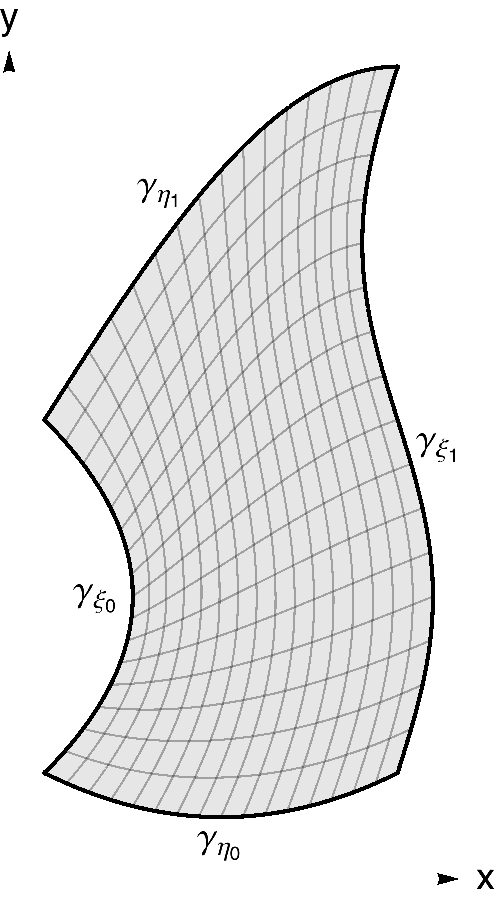
\includegraphics[width=.35\textwidth]{figs/testfig1.pdf}
\hspace{1cm}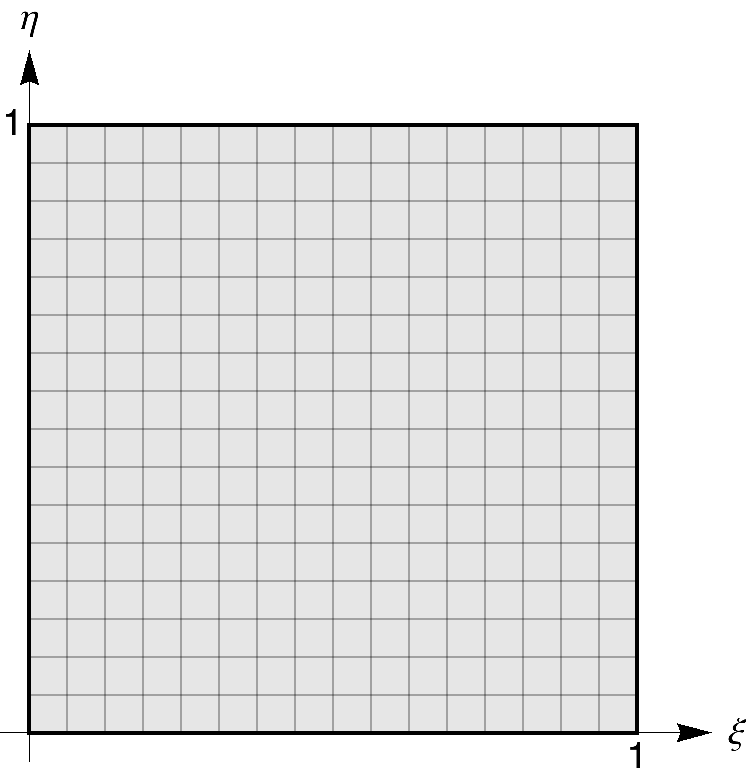
\includegraphics[width=.45\textwidth]{figs/testfig2.pdf}}
\caption{Figure Captions.}
\label{fig:label}
\end{figure}

\end{section}



%=== Appendix ============================================
\appendix

\dsp

\chapter{Appendix Title }{\label{appendix:a}}
\begin{section}{Section Title}

Appendicitis

\end{section}
\end{mainmatter}

%----- Bibliography ----------------
\ssp
\bibliographystyle{sty/JHEP3}
\bibliography{bib/thesis}

\end{document} 
